\documentclass[a4paper,12pt]{article}
\usepackage{fancyhdr}
\usepackage[ngerman,german]{babel}
\usepackage{german}
\usepackage[utf8]{inputenc}
\usepackage[active]{srcltx}
\usepackage{algorithm}
\usepackage[noend]{algorithmic}
\usepackage{amsmath}
\usepackage{amssymb}
\usepackage{amsthm}
\usepackage{bbm}
\usepackage{enumerate}
\usepackage{graphicx}
\usepackage{ifthen}
\usepackage{listings}
\usepackage{struktex}
\usepackage{hyperref}
\usepackage{tabularx}

\newcommand{\Fach}{Softwaretechnik I}
\newcommand{\Name}{Lukas Harsch}
\newcommand{\Matrikelnummer}{979272}
\newcommand{\Semester}{Wintersemester 2018/2019}
\newcommand{\Kapitel}{3}
\newcommand{\Titel}{Requirements Engineering allgemein}

\setlength{\parindent}{0em}
\topmargin 0cm
\oddsidemargin 0cm
\evensidemargin 0cm
\setlength{\textheight}{9.2in}
\setlength{\textwidth}{6.0in}

\hypersetup{
	pdftitle={\Fach{}: Kapitel \Kapitel{} - \Titel},
	pdfauthor={\Name},
	pdfborder={0 0 0}
}

\lstset{ %
	language=java,
	basicstyle=\footnotesize\tt,
	showtabs=false,
	tabsize=2,
	captionpos=b,
	breaklines=true,
	extendedchars=true,
	showstringspaces=false,
	flexiblecolumns=true,
}

\title{Kapitel \Kapitel}
\author{\Name{}}

\begin{document}
	\thispagestyle{fancy}
	\lhead{\sf \small \Name{}}
	\chead{\sf \small \Fach}
	\rhead{\sf \small \Semester{}}
	\rfoot{\sf \tiny Keine Gewähr auf Richtigkeit und Vollständigkeit}
	\lfoot{\sf \tiny Grafiken aus den Vorlesungsfolien\\CC BY-NC-SA }
	\begin{center}
		\LARGE \sf \textbf{Kapitel \Kapitel}\\
		\LARGE \sf \Titel
	\end{center}
	\vspace*{0.2cm}
	
	\section{Einführung und Motivation}
	\begin{itemize}
		\item Das RE ist eine Schlüssel-Phase in der System- und Softwareentwicklung, denn:
		\begin{itemize}
			\item Die meisten Fehler haben ihren Ursprung im RE
			\item Mängel im RE sind der wichtigste und häufigste Grund für einen Abbruch des Projekts
		\end{itemize}
		\item Deswegen: Primärer Ansatzpunkt für Verbesserungsmöglichkeiten eines Projekts
		\item Dadurch, dass das ganze Projekt auf dem RE beruht, breiten sich Fehler in den Anforderungen in späteren Phasen aus $\Rightarrow$ Lawineneffekt
		\item Kosten für eben diese Fehler in späteren Phasen steigen exponentiell
	\end{itemize}
	\begin{center}
		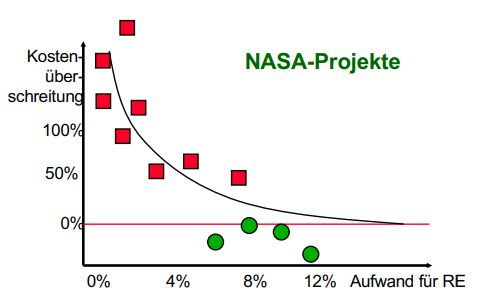
\includegraphics[width=\linewidth]{pics/nasa_re.jpg}
	\end{center}
	\begin{itemize}
		\item Mögliche Ma"snahmen zur Vermeidung:
		\begin{itemize}
			\item Methodische Erstellung der Anforderungsdefinitionen
			\item präzise Sprache verwenden
			\item automatische Werkzeuge verwenden
			\item Reviews
			\item schnelle Zyklen
		\end{itemize}
	\end{itemize}
	\section{Probleme des RE}
	\begin{itemize}
		\item \textit{Moving Targets} - Wechselnde Zielvorgaben
		\item Kommunikationsprobleme zwischen Beteiligten (\textit{Stakeholders})
	\end{itemize}
	\textbf{Konsequenzen:}
	\begin{itemize}
		\item Fehlverhalten von Systemen
		\item Unkontrolliertes Projekt-Management
	\end{itemize}

	\section{Grundlegende Begriffe}
	\subsection{Requirements Engineering (RE)}
	\begin{itemize}
		\item \textit{Requirements Engineering im weiteren Sinne:} Teildisziplin im Grenzbereich zwischen System Engineering, Informatik und Anwendungswissenschaften
		\item \textit{Requirements Engineering im engeren Sinne:} Gezielte Aktivitäten am Beginn eines System- oder Softwareprojekts zur Präzisierung der Problemstellung
	\end{itemize}
	\textbf{Ziele des RE} im engeren Sinne:\\
	Präzise, konsistente und vollständige Beschreibung aller Anforderungen an das System als Grundlage für anschlie"sende Systementwicklung.
	\begin{center}
		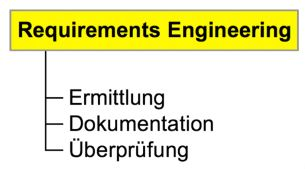
\includegraphics[width=8cm]{pics/re.jpg}
	\end{center}
	\subsection{Requirements Management (RM)}
	\begin{center}
		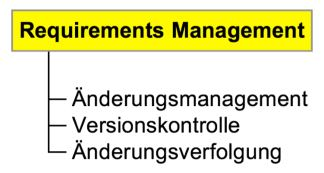
\includegraphics[width=8cm]{pics/rm.jpg}
	\end{center}
	\subsection{Anforderungen}
	
	\subsection{Anforderungsdokument}
	
	\section{Wesentliche Tätigkeiten des RE}
	
	\section{Formalismen, Methoden, Werkzeuge}
	
\end{document}